\documentclass{standalone}

%% for compilation with htlatex (to produce svg image),
%% uncomment the line below:
%\def\pgfsysdriver{pgfsys-tex4ht.def}

\usepackage{tikz}

\tikzstyle{tensor}=[rectangle,draw=blue!50,fill=blue!20,thick]

\begin{document}

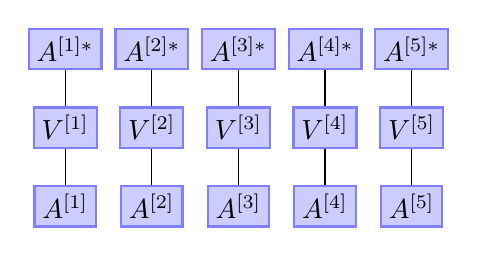
\begin{tikzpicture}[inner sep=1mm]
    \foreach \i in {1,...,5} {
        \node[tensor] (\i spin conjugate) at (1.1*\i, 1.) {$A^{[\i]*}$};
        \node[tensor] (\i) at (1.1*\i, 0) {$V^{[\i]}$};
        \node[tensor] (\i spin) at (1.1*\i, -1.) {$A^{[\i]}$};
        \draw[-] (\i) -- (\i spin);
        \draw[-] (\i) -- (\i spin conjugate);
    }m;
    \foreach \i in {1,...,4} {
        \pgfmathtruncatemacro{\iplusone}{\i + 1};
        %\draw[-] (\i) -- (\iplusone);
    };
    %\draw[-] (1.west) .. controls +(-1.5, 1) and +(1.5, 1) .. (5.east);
\end{tikzpicture}

\end{document}
